\section{Implementation}
\label{sec:impl}

We implement the design of Section~\ref{sec:bg} as one P4 program on a single Intel Tofino-1 switch,
with a control-plane configuration layer and a guarded control-test harness. This section starts with
an end-to-end walkthrough, then details each mechanism. For each mechanism we give the same account:
the problem it solves, the packet or state that triggers it, the observable effect, the failure
behavior, and the evidence that verifies it. Switch-internal names (ports, queues, tables) appear only
after the concept they implement.

\subsection{End-to-end walkthrough}
A read enters the switch from the master. The program records the request's arrival time, forwards the
request to the relay, and prepares to hold the relay's answer. When the acknowledgment and the
response come back, the program holds each in a switch queue and releases them at fixed offsets from
the recorded request time, so the master sees a constant CLRT; on release it replicates the response
and emits it as the two segments $[28,21]$. A control command is handled on a second internal path:
the SELECT prepares a hold, the OPERATE is admitted once and held, and it is released to the relay at
an internal delay, while the acknowledgment and echo the master sees are placed at fixed offsets from
the OPERATE's arrival. Two internal scheduling lanes keep the response path and the command path from
interfering. A single terminal decision applies every forwarding effect.

\subsection{Physical topology and packet paths}
The master reaches the switch on one port and the switch reaches the SEL-751 on another; these are the
only external cables. Three further ports are internal to the switch and carry no cable: two
recirculation paths give the response treatment and the control treatment their own scheduling lanes,
and one path is used by the switch's packet generator. The adversary observes only the master-facing
port; the relay-facing port and the internal paths are not observed. Fig.~\ref{fig:pipeline} shows the
detailed topology and names the internal ports and queues.

\begin{figure*}[t]
\centering
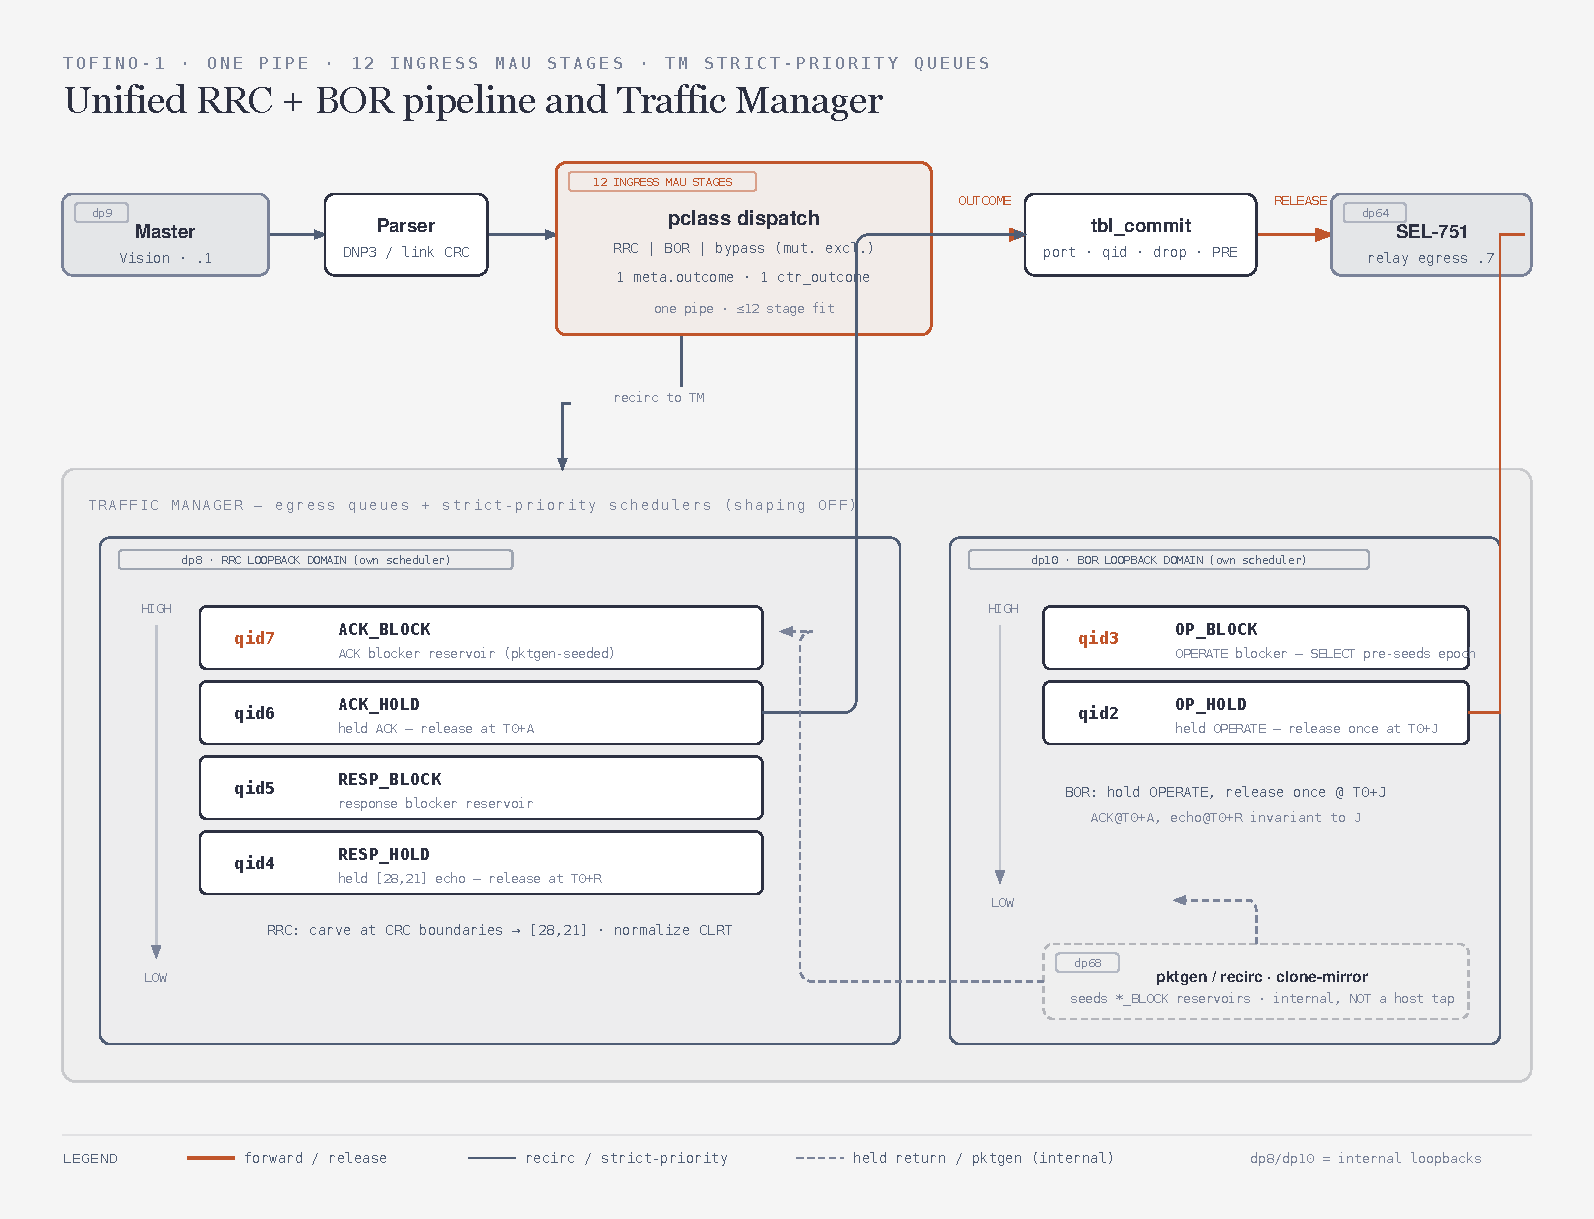
\includegraphics[width=0.95\textwidth]{figures/fig_pipeline}
\caption{Detailed switch pipeline. The parser and match-action stages compute one compact outcome that
a single terminal table applies; the Traffic Manager holds the response reservoirs and queues on one
internal lane (\code{dp8}) and the control queues on a second (\code{dp10}), with the packet generator
(\code{dp68}) seeding the reservoirs; egress carves the eligible response to $[28,21]$. Port and queue
names appear only here.}
\label{fig:pipeline}
\end{figure*}

\subsection{Recording the request time and arming deadlines}
\textbf{Problem.} A held packet must be released at a fixed offset from the request, but the switch has
no general-purpose timer. \textbf{Mechanism.} On the request (or the OPERATE), the program records an
ingress timestamp $T_0$ and arms two deadlines, $T_0{+}A$ for the acknowledgment and $T_0{+}R$ for the
response, from the policy offsets $A$ and $R$; the master-visible CLRT is then $R-A$. Anchoring to
$T_0$ rather than to the relay's later acknowledgment matters for the control command: because that
acknowledgment exists only after the held OPERATE is released, anchoring to it would leak the hold. An
offline model checks this anchoring against a mutant that arms the deadline at the acknowledgment, and
the mutant is killed.

\subsection{Reservoirs as data-plane timers}
\textbf{Problem.} Realize a deadline from packet scheduling alone. \textbf{Mechanism.} A held packet
waits in its queue behind a higher-priority reservoir of small ``blocker'' packets; a strict-priority
scheduler drains the blockers first, so the held packet cannot leave until its reservoir empties,
which the control plane sizes to the policy deadline. The switch's on-chip packet generator fills the
reservoirs and never generates master or relay traffic. Two generator profiles are distinguished by a
tag byte so that a read or select arm and a control hold trigger different reservoirs without
ambiguity.

\subsection{Response shaping: hold, release, replicate, carve}
Response shaping normalizes the timing and shape of an eligible 49-byte response. The acknowledgment
and the response are held in strict-priority queues and released at $T_0{+}A$ and $T_0{+}R$. On
release the program steers the response into the switch's packet-replication engine, which produces
two master-facing copies; egress then emits the 28-byte prefix from one copy and the 21-byte suffix
from the other, advancing the suffix's TCP sequence number by 28 so the two segments abut. The relay
produces the response; replication produces the two copies used for segmentation, and no clone
fabricates the response. By design the program edits no DNP3 byte and recomputes no DNP3 CRC, updating
only the IP and TCP checksums per segment; the hardware evidence bounds this to a sequence-contiguous,
CRC-valid, checksum-valid 49-byte reconstruction, not byte identity to a source frame. The 49-byte
frame is a 10-byte link header, an 18-byte first data block (16 data + 2 CRC), a second 18-byte block,
and a 3-byte final block; byte~28 falls between the first and second blocks (Fig.~\ref{fig:carve}).
TCP may segment a byte stream at any offset, so cutting at byte~28 is a design and verification
choice that keeps each segment aligned to a completed CRC block, not a TCP requirement.

\begin{figure}[t]
\centering
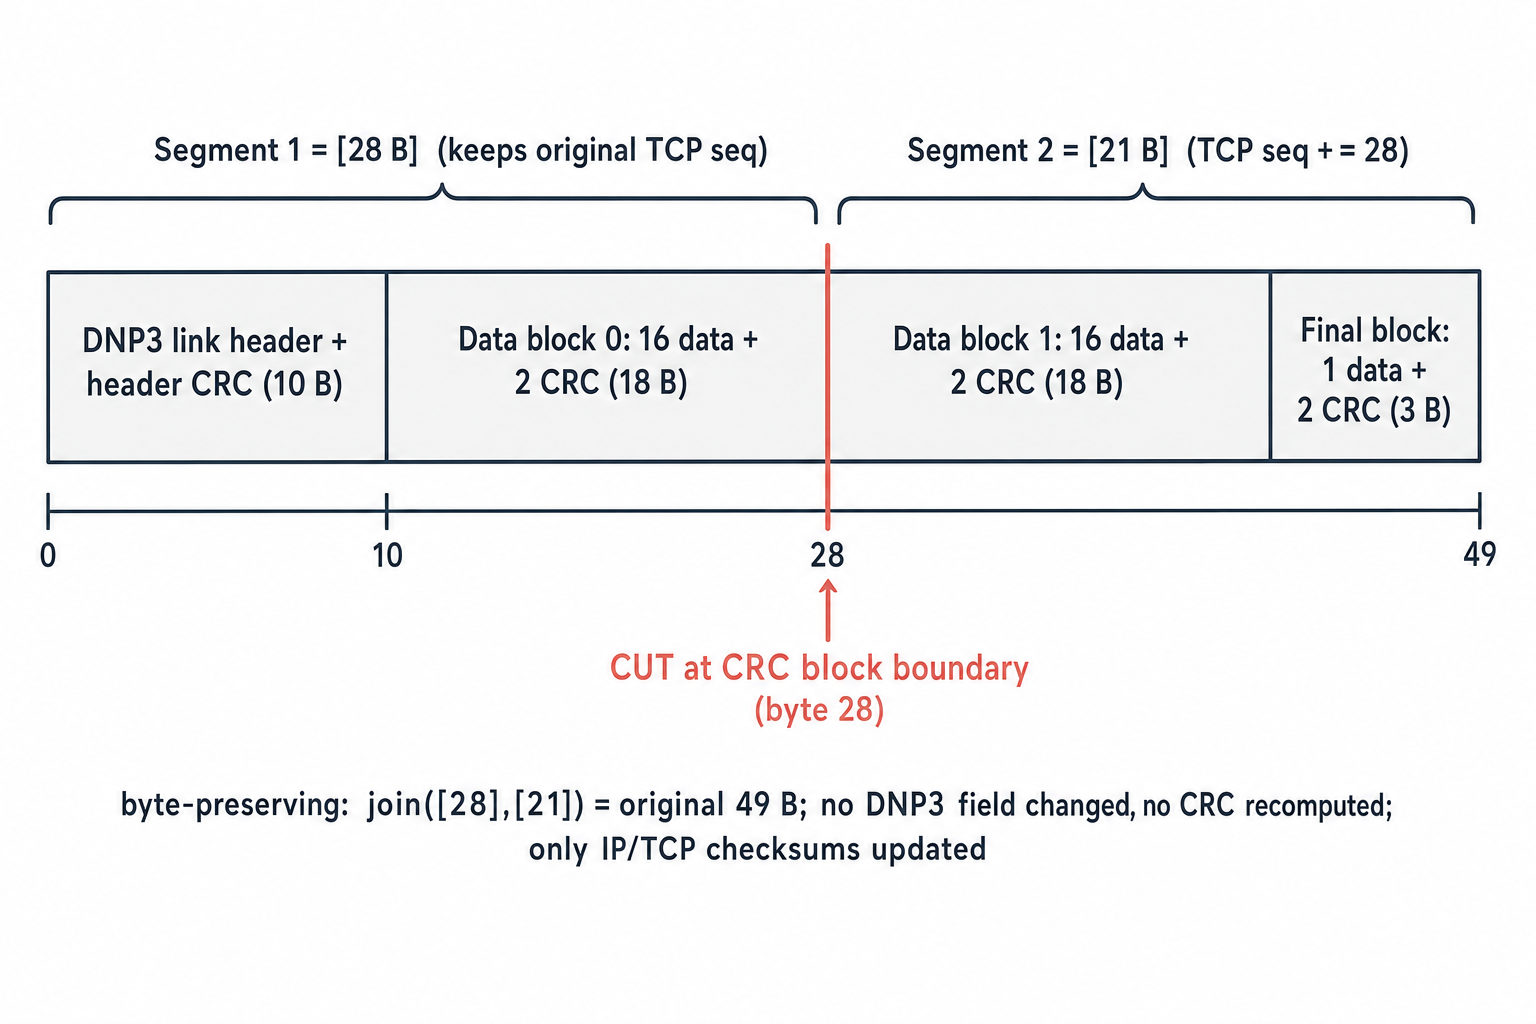
\includegraphics[width=0.98\columnwidth]{figures/fig_carve}
\caption{The 49-byte response and the $[28,21]$ carve. The cut at byte~28 is a boundary DNP3 already
places between CRC-protected blocks; the prefix keeps the original TCP sequence number and the suffix
advances it by 28. No DNP3 byte is edited and no DNP3 CRC is recomputed.}
\label{fig:carve}
\end{figure}

\subsection{The control command and its state}
\textbf{Problem.} An outbound OPERATE exposes an operation-timing fingerprint, and releasing it on a
fixed schedule would still reveal it. \textbf{Mechanism.} The SELECT prepares a hold by seeding the
control reservoir, so the hold is armed before the OPERATE arrives. The switch admits one matching
OPERATE, holds it, and releases it once to the relay at an internal delay drawn in the data plane from
a bounded set. The master-visible acknowledgment and echo are released at $T_0{+}A$ and $T_0{+}R$,
anchored to the OPERATE's own arrival and independent of the internal delay, so the observable gap
carries no information about it. After release the transaction's generation is kept as a spent marker
until the next SELECT; a retransmitted OPERATE that reads the spent marker is treated as a duplicate
and dropped. \textbf{Evidence boundary.} The hardware captures establish the master-visible placement
and the delay-invariant gap; the offline model verifies the single release; the relay-facing release
time and the number of copies delivered are not captured, so single release is modeled, not measured.

\subsection{Two independent scheduling lanes}
Response shaping seeds acknowledgment and response reservoirs on high-priority queues. On one shared
strict-priority schedule these reservoirs starve the control hold that would sit below them, shifting
its release toward the response's release time instead of its own deadline
(Fig.~\ref{fig:scheduler}a). The design places the response queues on one internal recirculation lane
and the control queues on a second (Fig.~\ref{fig:scheduler}b), so each arbitrates on its own
scheduler. A register-domain separation keeps a control-path packet from touching the response path's
state. Both lanes are internal to the same switch and the same program.

\begin{figure}[t]
\centering
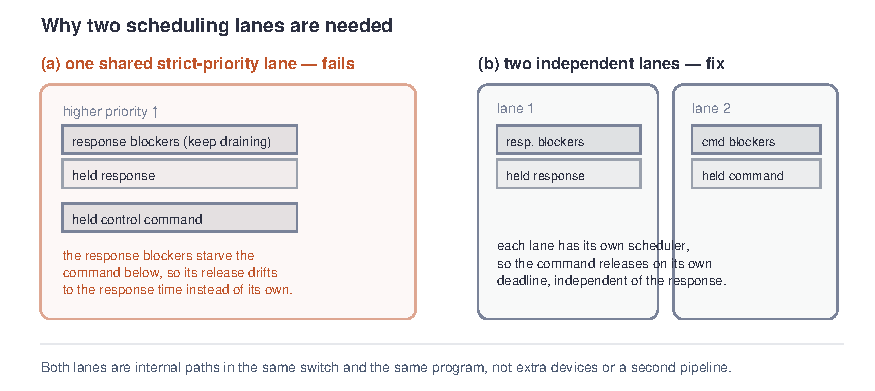
\includegraphics[width=0.98\columnwidth]{figures/fig_scheduler}
\caption{Why two scheduling lanes are needed. (a) On one shared strict-priority schedule, the
response's blocker packets starve the held control command below them, so its release drifts to the
response's release time. (b) Two independent lanes each carry their own blockers and held packet, so
the command releases on its own deadline. Both lanes are internal to the same switch and program.}
\label{fig:scheduler}
\end{figure}

\subsection{One outcome, one commit}
Earlier match-action stages compute one compact result and a single terminal table applies it. The
terminal table is keyed on that result and is the only stage that sets the egress port, the queue, a
drop, a bypass, or a multicast group; every defined result is mapped by a constant entry. The default
action, taken only for the otherwise-unreachable unset result, forwards the packet unmodified rather
than dropping it. This is distinct from the explicit dispositions of recognized traffic: internal-only
packets such as a bad-port packet, a returning generator token, a clone, a duplicate response, or a
retired blocker are mapped to an explicit drop, while a recognized but ineligible or unsupported
response is mapped to an explicit forward. The single-table structure keeps the disposition auditable
and, with a flattening of the decision logic into two mutually exclusive tables that co-place in one
stage, lets the whole program fit one ingress pipeline within its stage budget.

\subsection{Control plane, failure behavior, and safety}
The control-plane layer brings up the ports, creates the queues at descending strict-priority levels
with shaping disabled, installs the multicast group and the generator profiles, writes the timing
parameters and the internal-delay set, and initializes the state. Every write is read back and
compared, and a mismatch or a configuration warning leaves the mechanism disabled rather than
partially configured; there is no configuration snapshot, and rollback is a forward, readback-checked
teardown to a plain forwarding state. Traffic outside the eligible class, unsupported functions, and
malformed frames are forwarded unchanged. The control-test harness that issues a physical SELECT and
OPERATE is guarded: it permits only two isolated control points and refuses a breaker-close point.
Across every guarded transaction all 32 relay outputs remained open and no breaker operation was
attempted.

\subsection{Resource fit and limitations}
The program compiles for one Tofino-1 ingress pipeline within the twelve-stage match-action budget.
The evaluation is on physical hardware, one switch and one relay; it is not a deployment study. The
implementation does not observe the relay-facing link, does not normalize total response length, and
is evaluated on one outstation and one eligible response class; Section~\ref{sec:eval} reports the
measured consequences of these bounds. The loaded source and binary are identified by hash, the
analysis regenerates deterministically from the captured traces, and a manifest verifies every derived
artifact.
